\chapter{Data analysis examples}~\label{appendix-data-analysis-examples}

\epigraph{A sample of the manifold}{anon}

\begin{figure}
    \centering
    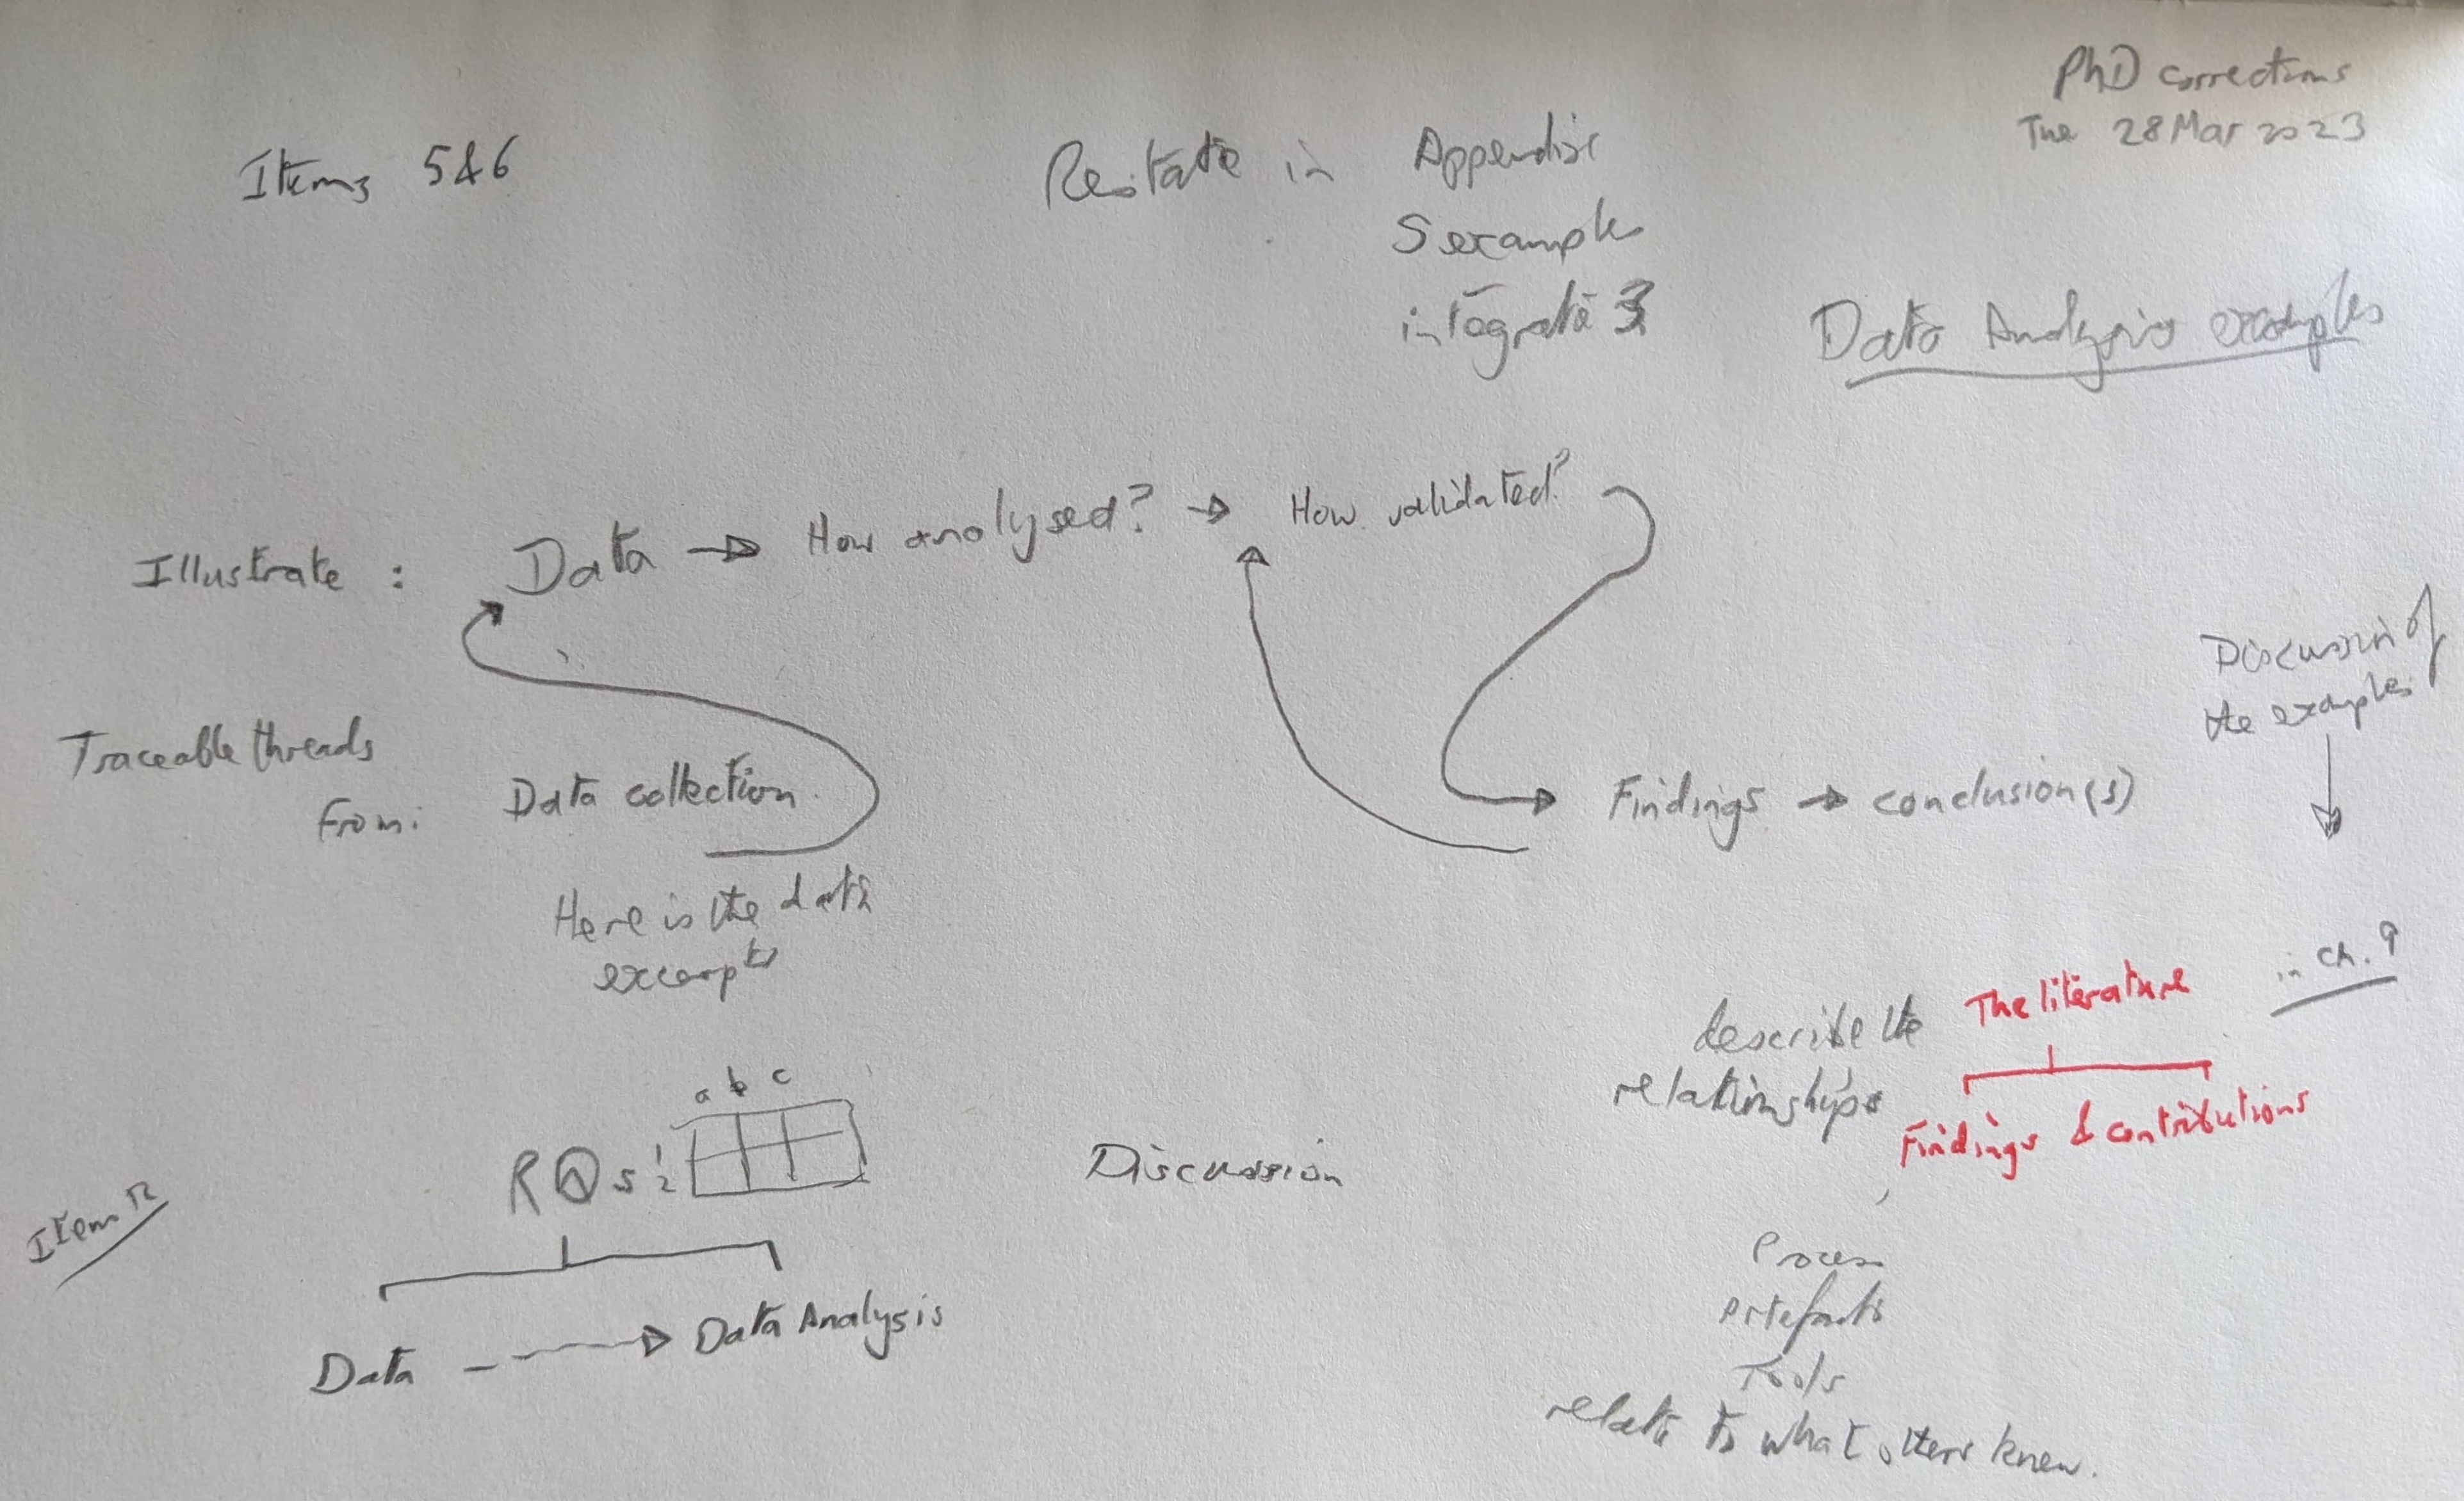
\includegraphics[width=\textwidth]{images/rough-sketches/worked-examples-in-context.jpg}
    \caption{Addressing - in part - items 5, 6, and 12}
    \label{fig:worked-examples-in-context}
\end{figure}

\section*{Context}
Items, 5, 6, and 12 in \secref{report-to-candidate-section} are repeated below, this appendix aims to address these items. Figure \ref{fig:worked-examples-in-context} illustrates my mapping of the connections and interactions that emerge from these items. Here a range of worked examples are provided for the interested reader, they reflect the approach and analysis of a multitude of findings that arose as part of this research. The mappings of findings are maintained using the spreadsheet design described in \secref{appendix-thematic-analysis}.

\begin{enumerate}
    \item[5] Clarify the data that was collected at each case study and how it was analysed and how it was validated, with illustrative data provided throughout.
    \item[6] More information is needed to clarify the research process i.e., to provide a clear link between the data collected, the findings and the conclusions drawn.
    \item[12] Provide more detail in the Appendices of the data and the data analysis done in relation to the RQs.
\end{enumerate}

\subsection*{Structure of each example}
The examples follow a consistent workflow which has been simplified to make the narrative clearer, the actual workflows for examples often included additional iterations, for example as more data was collected (some data arrived on an ongoing basis and bolstered with research-in-progress).

The structure is:

\begin{enumerate}

    \item Data, including how it was collected 
    \item Analysis, including how it was analysed
    \item Findings, and how they were validated
    \item Conclusions
\end{enumerate}

Candidate examples include:
\begin{itemize}
    \item \myindex{Kiwix} hackathon in Stockholm: where small changes led to an immediate and material improvement in reliability. 
    \item \myindex{Kiwix} experiment pre and post the hackathon: where comparisons in the experiment and the control apps indicate the improvements in reliability were achieved as a direct effect of making and releasing improved versions of apps.
    \item \myindex{PocketCode}\index{Catrobat} hackathon in Graz: this corroborates the pattern of results during and post hackathon. The results diverged from Kiwix after several months.\sidenote{Perhaps this could go before the Kiwix experiment, TBD}. In the discussion chapter incorporate the examples of how Moonpig actively managed reported crashes from Robospice, and from two homegrown bugs.
    \item Commercial project (\myindex{C1}): from release management reports through coding suitable tests, applying fixes, deploying the improved release. Also, third-party libraries (\myindex{OkHttp} in this example) deserve respect and attention to detail.\index{Third-party libraries!OkHttp}
    \item Three examples of scheduled automated emails from mobile analytics services (Sentry, Fabric Crashlytics, and whatever the one is that's eluding my memory right now). Also introduce Android Vitals automated emails and their infrequency. Cross referencing with Android Vitals reports. (via: \myindex{LocalHalo}, \myindex{Catrobat})
    \item Microsoft App Center's reports of future crashes. (via \myindex{C1}, \myindex{Micro experiments})
    \item Better bug reports by incorporating content from mobile analytics dashboards, including longevity of the contents of reports. (via \myindex{C1}, \myindex{Kiwix}, \myindex{GTAF}, and others).
    \item Coping with new Android releases using mobile analytics: \myindex{Moonpig}, \myindex{Third-party libraries!Robospice}, \myindex{SmartNavi}.
    \item \myindex{LocalHalo} \myindex{React Native!Expo framework} and the measurements performed by two mobile analytics services: \myindex{Sentry} and \myindex{Android Vitals} during the runtime problems.
\end{itemize}

\section{Kiwix hackathon in Stockholm}

\section{}